\documentclass[12pt]{article}
\usepackage{graphicx}

\begin{document}
  \noindent \textbf{Daniel Alabi and Cody Wang} \\
  \textbf{CS 324}
  \hfill

  \begin{enumerate}
  \item[1] \textbf{Standardizing the data is a terrible idea, in this case,
    because:}
    \begin{enumerate}
      \item The goal of standardizing the columns is to modify the data so that their units are considered consistent. In this case, the units for each column are the same and standardization won't solve the problem of the skewedness in the data.
      \item Standardization usually works on data with a normal distribution, but the data here is skewed. Standardizing using the z-score centers the points around the mean, which is not what we want.

    \end{enumerate}
    
  \item[2] \textbf{The method for handling empty clusters reduce the clustering error because:}

    Assume there are $n$ empty clusters ($e_1, e_2, \ldots, e_n$) in the dataset. We obtain the points that have the greatest
      SSE (\textbf{S}tandard \textbf{S}quares \textbf{E}rror), which are points
      that are farthest away from their assigned centers. Let these points be
      $p_1, p_2, \ldots, p_n$ with initial centers $c_1, c_2, \ldots, c_n$. 
      
      Next, our procedure replaces each $e_i$ with $p_i$ making $e_i=\{p_i\}$
      (cluster of one point). At this juncture, the total SSE of the data
      reduces by $(p_1-c_1)+\ldots+(p_n-c_n)$. 
      
      The next step is to re-run
      k-means. Some more points in the dataset might be assigned to any of
      $e_1, \ldots, e_n$ in this iteration. Call these points, $x_1, \ldots, x_m$ previously assigned
      to centers $d_1, \ldots, d_m$. This means
      that all $x_i$ are now closer to some $e_j$ which reduces the 
      total SSE by $(x_i-d_i)-(x_i-e_j) > 0$ for each $i$.
      Therefore, our strategy strictly reduces the clustering error. 
    
    \item[3] \textbf{Determining the ``best'' value of $k$}: 
      \begin{enumerate}
      \item By choosing a $k$ number of clusters so that adding another cluster doesn't give much better modeling of the data, we would obtain the “best” value of $k$. We plotted the total clustering error vs. $k$ and estimated that the ``knee'' of the graph (after which point an increase in $k$ does not give a much lower SSE) is $k=4$ (Figure 1). 
        \begin{figure}[h]
          \centering
          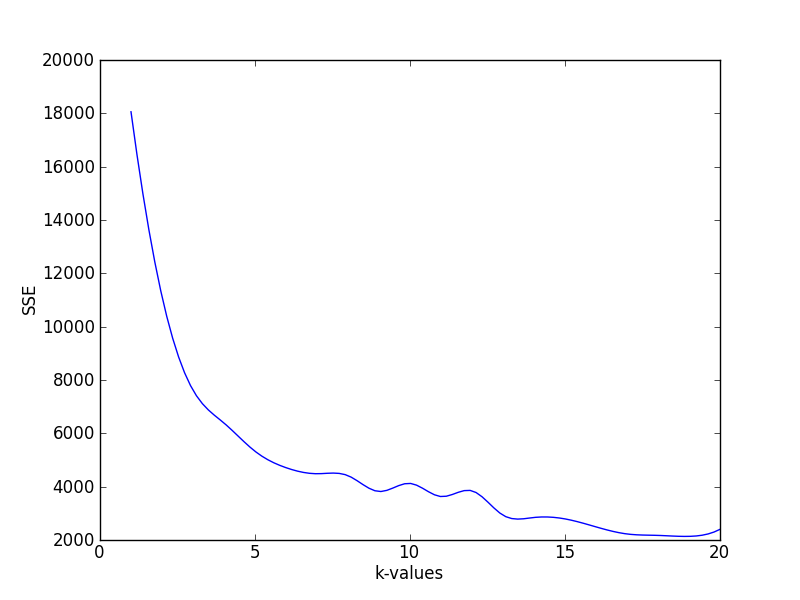
\includegraphics[width=0.80\textwidth]{SSEvsK-values.png}
          \caption{Total clustering error vs. k-values}
        \end{figure}
      \item The four centers we found when $k=4$ using the random method are:
        \begin{enumerate}
          \item \[6.1733139930, 2.850698311, 1.275054902, 2.2216898386041644\]
	  \item \[1.1402166700, 0.120837269, 0.241610808, 0.13463948847174742\]
	  \item \[10.040470088, 7.690923877, 5.475507216, 7.34666421346101\]
	  \item \[3.66942917, 0.24139948309, 0.280561013, 0.187318590906642\]
            \end{enumerate}
    The pairwise distances between the four centers are quite large and differentiable, indicating that they are distinguishable from each other. Thus, we consider $k=4$ a “best” $k$-value.
      \end{enumerate}

    \item[4] \textbf{Interpretation of cluster centers}:
      Cluster centers for $k=5$ using the random method:
      \begin{enumerate}
        \item $C_1$: 9.205200508007167, 6.549592418865086, 4.382863104502213, 6.05400809985096
        \item $C_2$: 1.1957883896658879, 0.2831857287688855, 0.6773784717388026, 2.442853448334277
        \item $C_3$: 0.14578024655008265, 0.38863504103029645, 1.016633382170557, 0.23717237150543677
        \item $C_4$: 1.6533165770665175, 0.06027800449329119, 0.03643387226381733, 0.02126572113032895
        \item $C_5$: 4.686396688802443, 0.7722908086220749, 0.5432474660336377, 0.5337653026154968
          \end{enumerate}
          $C_1$ represents the users that have made significant amount of edits in all four Wikipedia namespaces.\\
          $C_2$ represents the users that have made some amount of edits in the main and the user talk namespaces, and relatively few edits in the other namespaces.\\
          $C_3$ represents the users that have made some amount of edits in the user pages, and relatively few edits in the other namespaces.\\
          $C_4$ represents the users that have made some amount of edits in the main article and little or no changes in the other namespaces.\\
          $C_5$ represents the users that have made a significant amount of edits in the main article and relatively few in the other namespaces.

    
  \end{enumerate}
\end{document}
